\subsection{Fórum}
O desenvolvimento da página de fórum trouxe diversas dificuldades entre elas a gestão de filtros e pesquisas e também a mostragem de publicações e atualização das mesmas.


\vspace{10mm}
\begin{figure}[htb]%
  \centering
  \subfloat[\centering Página de forum]{{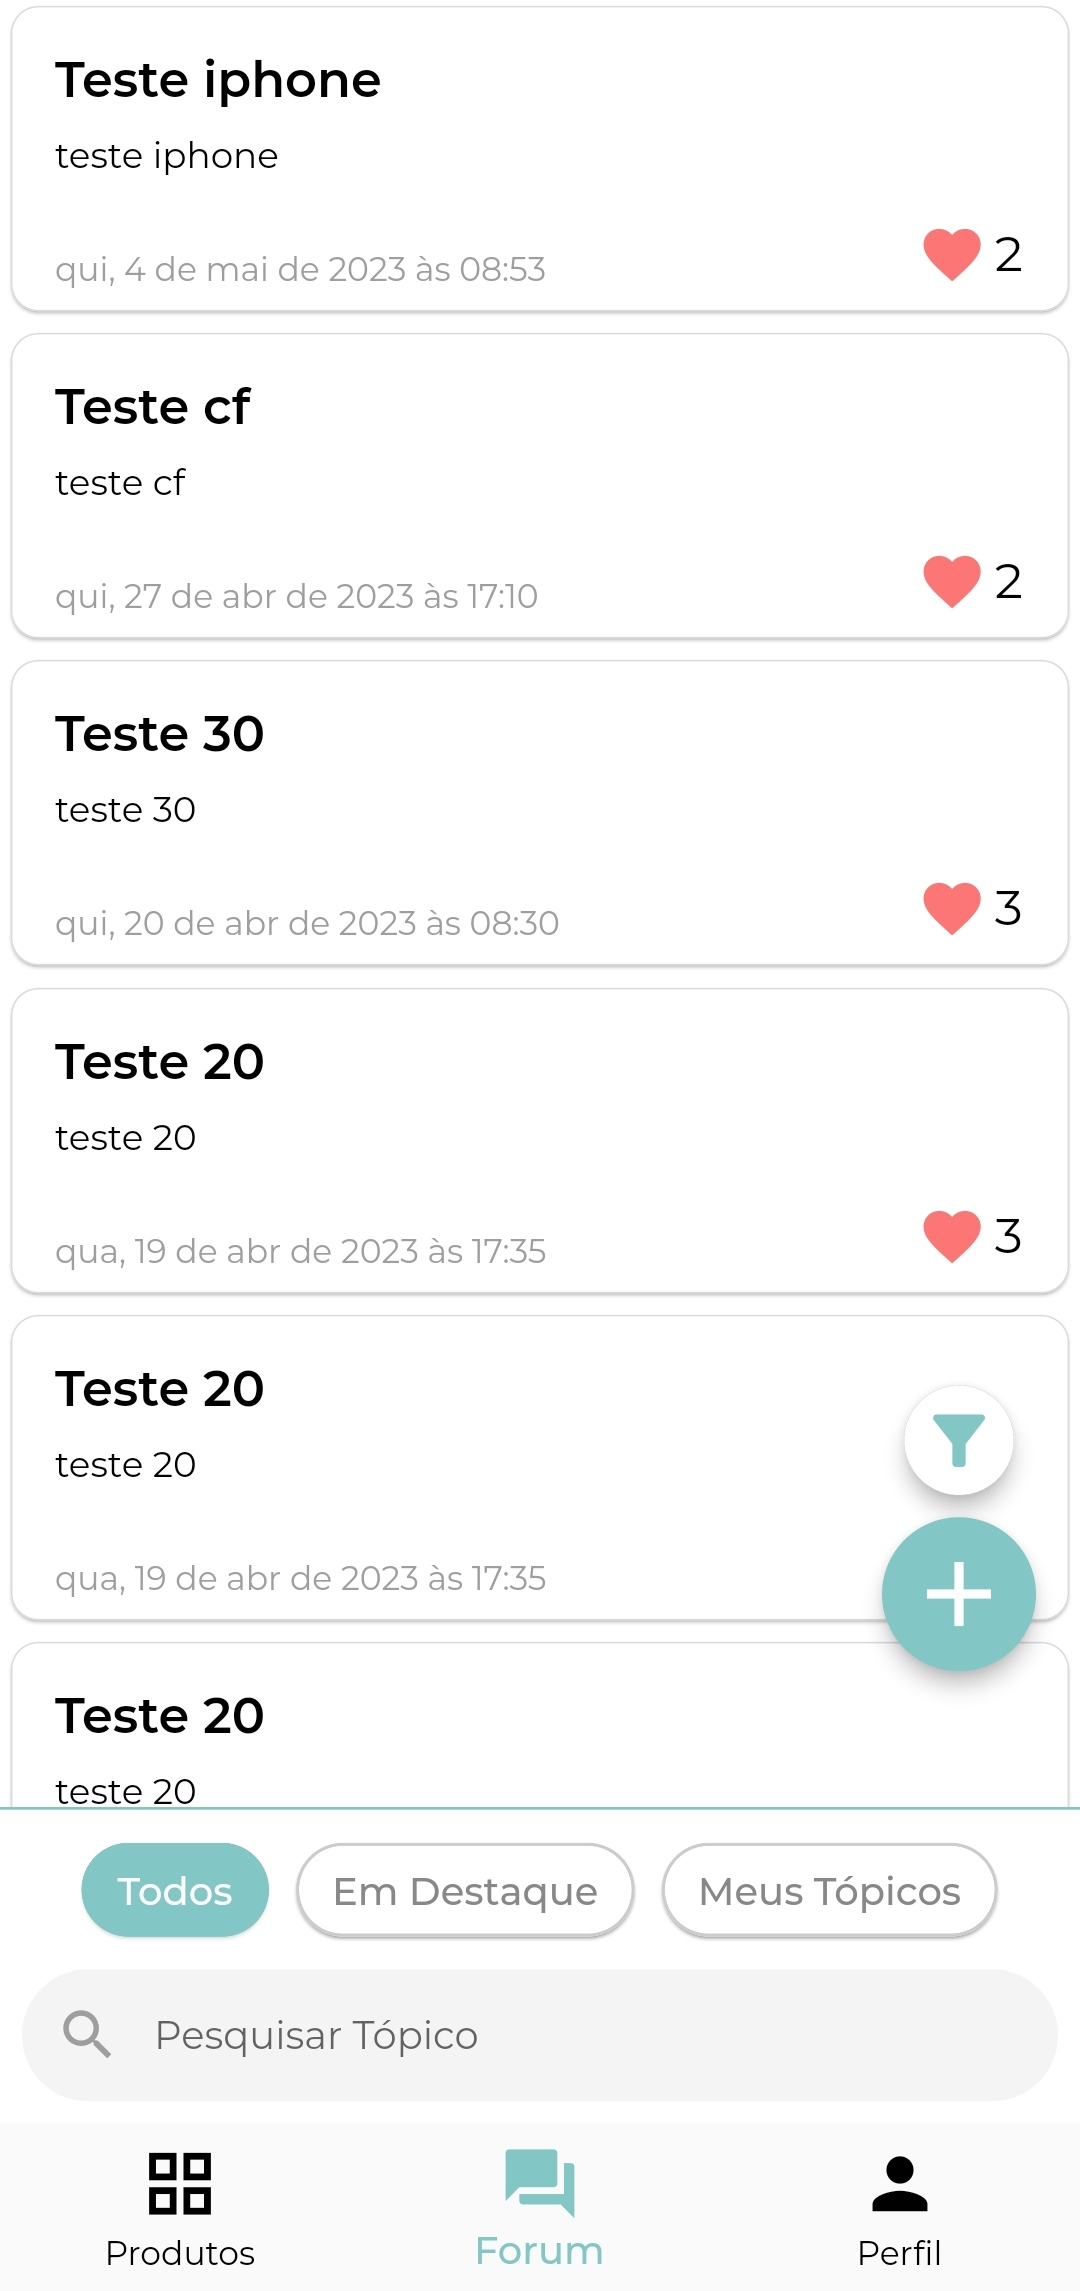
\includegraphics[width=0.3\textwidth]{images/implementacao/frontend/forum/1686055611203.jpg} }}%
  \qquad
  \subfloat[\centering Filtragem de tipo]{{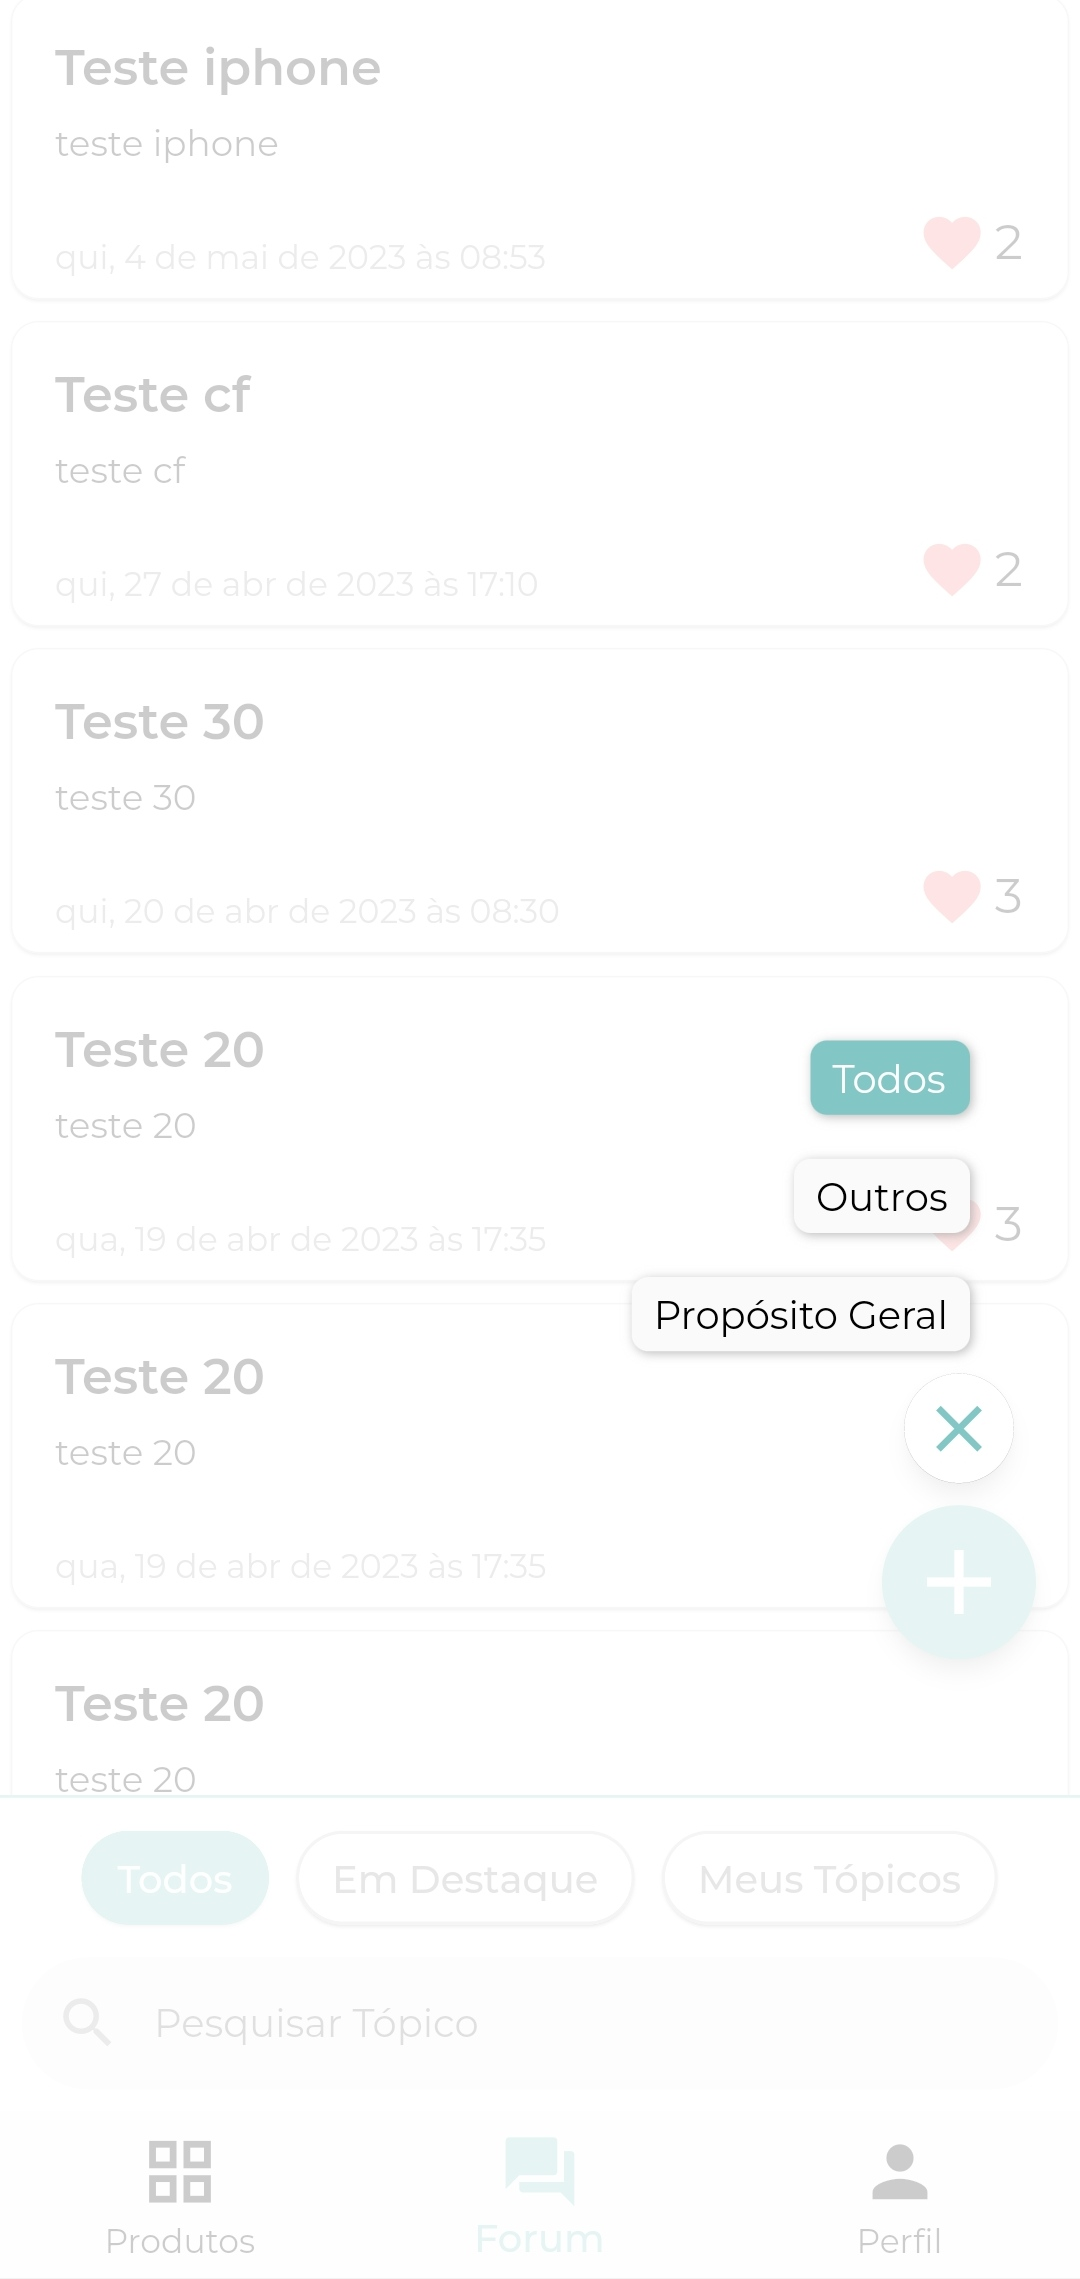
\includegraphics[width=0.3\textwidth]{images/implementacao/frontend/forum/1686055611213.jpg} }}%
  \label{fig:72}%
\end{figure}
\vspace{10mm}

\newpage

\subsubsection{Filtragem de tópicos}
O grande problema com a filtragem dos tópicos é que existem 3 tipos de filtros, o filtro de categoria de tópico, o filtro de tipo de tópico e o filtro de pesquisa. 

Uma vez que algum filtro seja alterado, os filtros seguintes deverão ser novamente executados de forma a garantir que todos estes se encontram aplicados, inicialmente este tipo de filtragem não era executado, o que levava a problemas como por exemplo sempre que se efetua uma pesquisa, esta não era efetuada sobre as publicações filtradas o que levava a que a pesquisa fosse efetuada por todas as publicações.

Outro problema encontrado era na troca de categoria, por vezes acontecia que os filtros de categoria adicionavam-se o que levava a que estes não mostrassem publicações.

Sendo assim foram criados métodos para auxilio na filtragem, assim como também uma prioridade, sendo que a cada método invoca o método seguinte em forma de encadeação. Primeiramente aplica-se o filtro de categoria, de seguida este envia o resultado da filtragem para o método de filtragem por tipo e por fim se existir algum tipo de pesquisa os tópicos serão filtrados pela mesma.

\begin{figure}[htb]
  \centering
  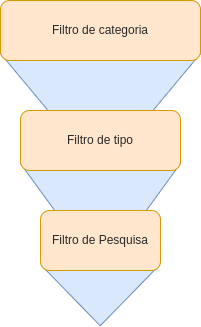
\includegraphics[width=0.25\textwidth]{images/implementacao/frontend/forum/filtros/filtros.png}
  \caption{Filtragem do forum}
  \label{fig:73}
\end{figure}

\newpage

\subsubsection{Carregamento de tópicos}
Inicialmente o carregamento de tópicos fazia-se por inteiro, desde carregamento de todos os tópicos, até ao carregamento de todos os dados dos mesmos, pois visto que não existiam muitos tópicos este não seria um problema para a API, mas conforme os testes foram sendo realizados a quantidade de tópicos existentes foi sendo incrementada, sendo possivel visualizar o tempo de demora de resposta do servidor a aumentar, assim como também a performance da aplicação no fórum a piorar.

De forma a resolver este problema primeiramente pensou-se em uma técnica de sliding window no total, o problema é que esta solução iria levar a que se o utilizador desejar voltar para trás nos tópicos a partir de uma quantidade escolhida de tópicos estes teriam de ser carregados novamente, o que não levaria a uma boa experiência de utilização.

Para resolver este problema foi utilizada a ideia de sliding window, mas os tópicos iriam se manter carregados, sendo que a própria framework consegue através da lista retirar de renderização os tópicos que o utilizador não consegue ver. 

Esta solução foi implementada utilizando 3 valores, quantidade de tópicos a obter, índice inicial e data do primeiro tópico. O valor de quantidade de tópicos a obter, inicialmente 10, permite limitar a quantidade de tópicos que a API irá processar reduzindo o tempo de resposta, o índice inicial, permite indicar qual o índice do primeiro elemento que se deseja obter da lista e a data do primeiro tópico permite manter uma referência temporal para obter tópicos, garantindo assim que a lista que se está a visualizar é sempre a mesma.

\begin{figure}[htb]
  \centering
  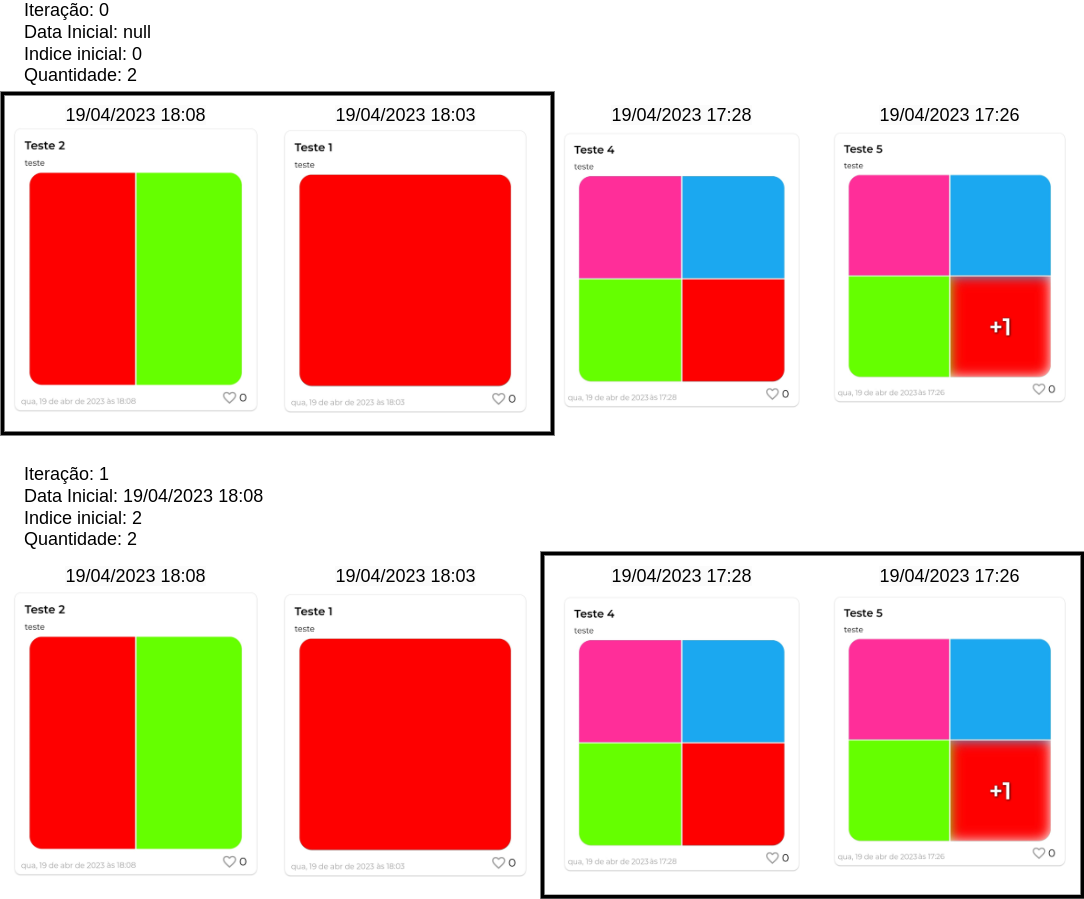
\includegraphics[width=0.5\textwidth]{images/implementacao/frontend/forum/loading_topics/topics_loading.png}
  \caption{Carregamento de tópicos}
  \label{fig:74}
\end{figure}

Foi também reduzido a quantidade de dados carregados por cada tópico, sendo assim apenas os comentários diretos à publicação são carregados não carregando as respostas a estes, o que também contribuiu para a melhoria de performance.

Por fim sempre que o utilizador alcança o fim da lista de tópicos este poderá deslizar para carregar mais tópicos.

\newpage

\subsubsection{Detalhes de tópico}

A página de detalhes de tópico sofreu os mesmos problemas que a página anterior sendo necessário aplicar a mesma solução sobre os comentários de tópico e também sobre as respostas ao mesmo. Sendo assim são carregados os primeros 10 comentários e por fim mostrado ao utilizador quantos mais comentários existem que poderá carregar sendo o limite 10 comentários.

Estes comentários podem também conter respostas sendo que estas podem ser carregadas também 10 de cada vez conseguindo o utilizador esconder ou mostrar estas.

Um problema que surgiu no desenvolvimento da página de detalhes de tópico foi também o destaque de uma mensagem para por exemplo destacar alguma resposta de um notificação. Este foi um grande problema pois com a nova implementação as mensagens não se encontram carregadas no momento de destacar a mensagem, pelo que e necessário procurar a mesma dentro das mensagens carregadas, expandindo assim as respostas do comentário que contêm a mensagem a destacar.

O destacamento de mensagens também continha um erro no qual sempre que algo no ecrã e atualizado, este recarregava a animação pelo que este código teve de ser movido de forma a apenas ser executado no momento de inicialização do ecrã após todos os elementos se encontrarem devidamente carregados.

\begin{figure}[htb]
  \centering
  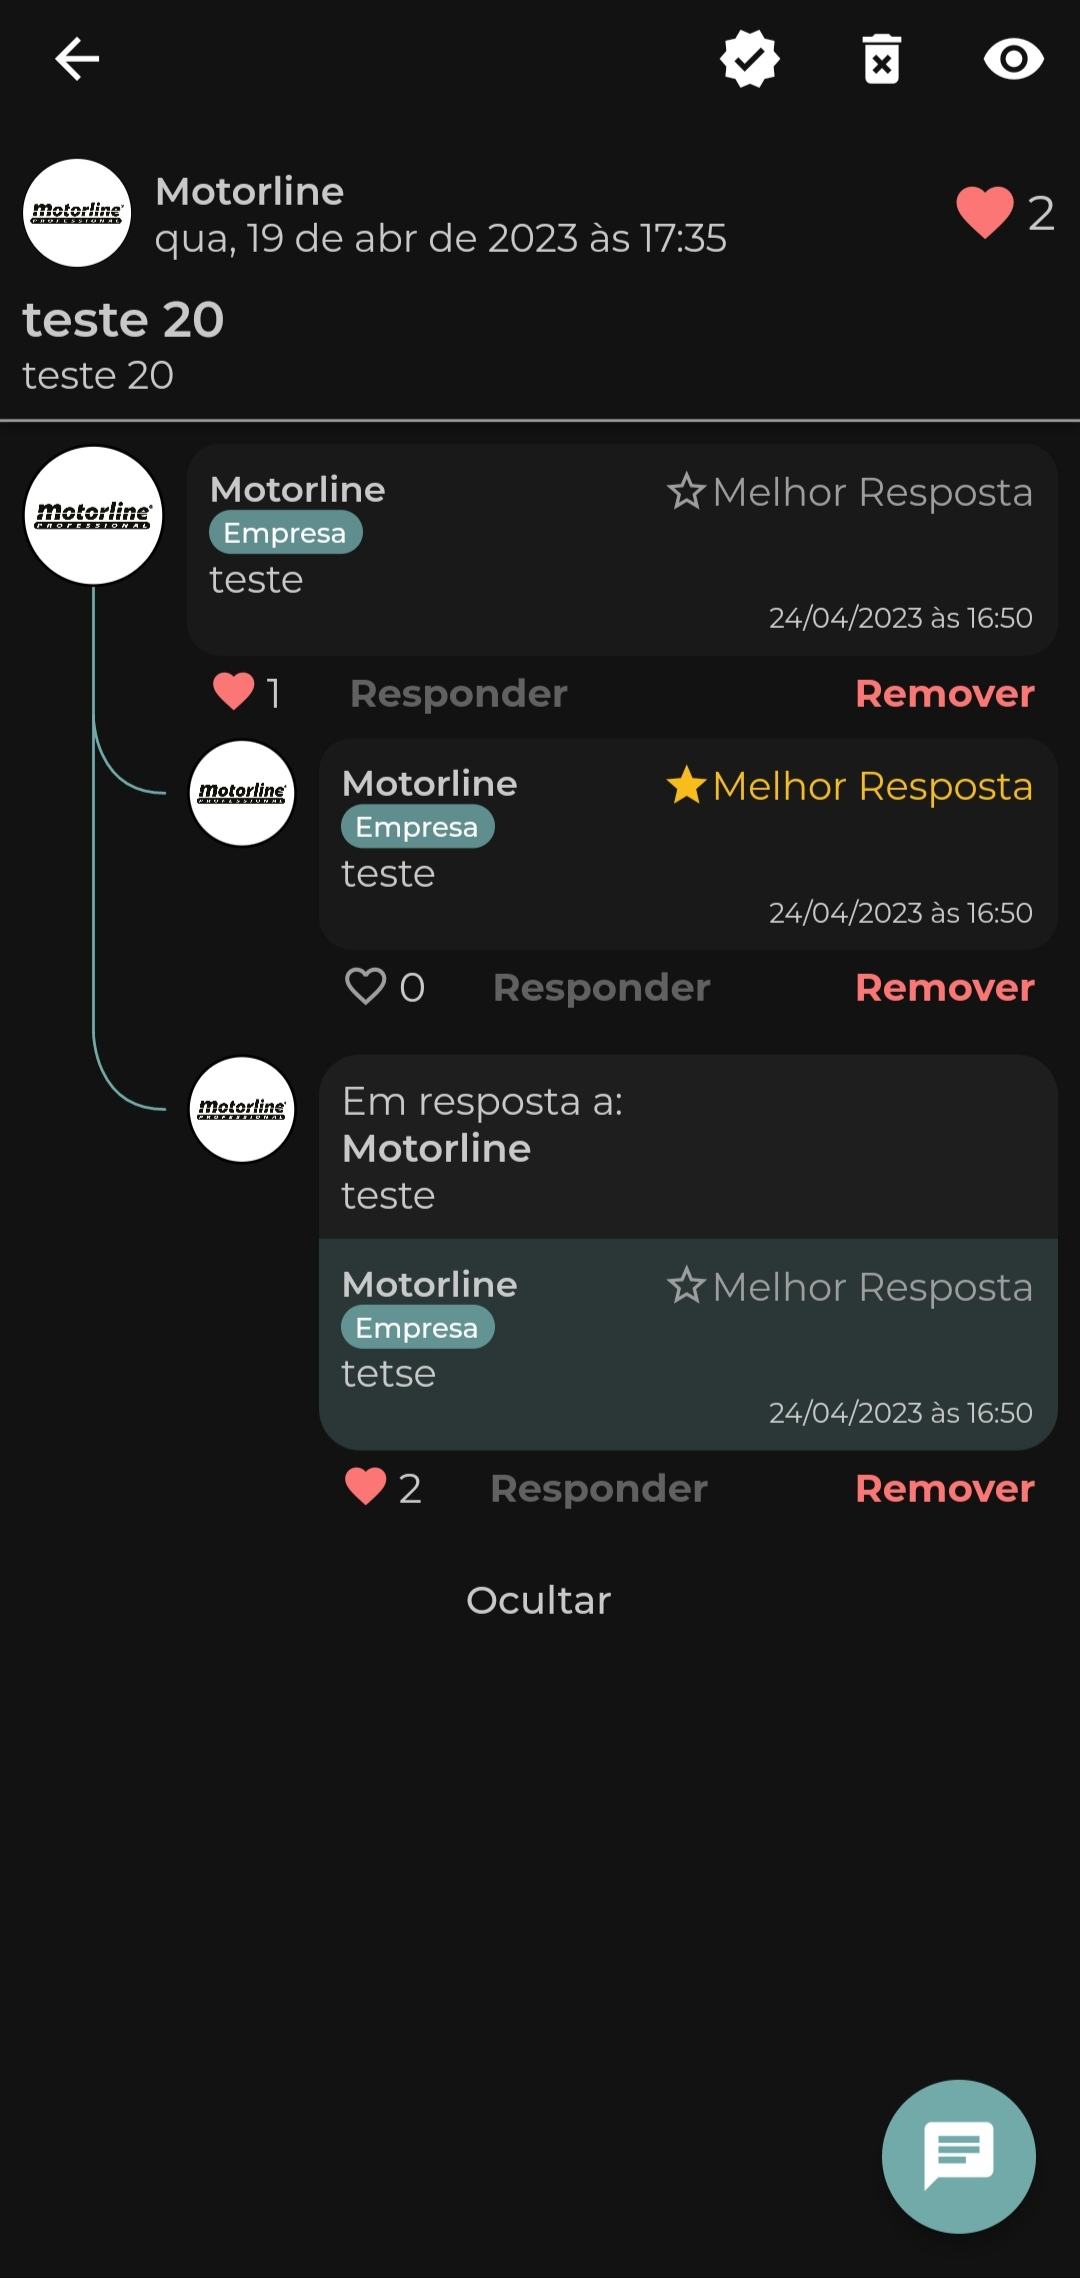
\includegraphics[width=0.35\textwidth]{images/implementacao/frontend/forum/loading_topics/1686062701127.jpg}
  \caption{Destaque de mensagens}
  \label{fig:75}
\end{figure}